\chapter{Sprint 3}

\minitoc

\subsubsection{Purpose}

This chapter will outline the work we did in the third sprint. It explains in detail how we planned the sprint, including which user stories we chose and the architecture we employed to implement these. Details on the implementation on each user story is also included, as well documentation on the testing process. Finally our evaluation of the third sprint is presented. 

\clearpage

\section{Planning}

\subsection{Duration}
This sprint started on October 22th and lasted for two weeks. A customer demo was held at the 1st of November to show of what we had achieved during the sprint and to ensure that the customer agreed with the solutions and the direction we were going in.

\subsection{Sprint Goal}
The goal for this sprint was to redesign the system to accomodate the new wishes from the customer, and to present a working protoype incorperating the suggested technologies at the end of the sprint.

\subsection{Sprint Backlog}
The user stories included in the sprint backlog is presented in Table~\ref{table:sp3backlog}. As we chose to accomodate the new wishes from the customer we were forced to use a considerable amount of time on reasearch on new technologies and on redesigning the system to utilize these technologies. As a result the amount of time available for implementation of user stories was reduced, and this time we only had 50 hours available for this purpose. From experiences from the previous sprints, we tried to make each user story concise and not too general. We feel this helped us a lot in estimating the user stories more accuratly than in previous sprints.

\begin{table}
\caption{Sprint 3 Backlog}
\centering
\begin{tabular}{ l p{8cm} l l }
\hline 
			&				&\multicolumn{2}{c}{Hours}			\\
 User Story	& Short Description		&Est.		&Act.	                               \\ 
\hline \\ [-2.0ex]
 
\bf{1}     &\bf{Navigate the application like a directory}		&\bf{6}		&\bf{4.5}          \\ 
		  &Decide on syntax						&			&		\\
		  &Detect and parse navigation commands	&			&		\\
		  &Change directory when command is issued&			&		\\
		  &Testing							&			&		\\
		  &Documentation						&			&		\\

 \bf{2}     &\bf{Store variables in the console} 				&\bf{5}		&\bf{4}               \\ 
		  &Make objects in current directory available		&			&		\\
		  &Ensure persistent storage of the stored objects	&			&		\\
		  &Testing								&			&		\\
		  &Documentation							&			&		\\

 \bf{3}     &\bf{GUI represent current directory} 			&\bf{5}		&\bf{4}		     \\ 
		  &Make viewsfor each directory in CouchDB		&			&		\\
		  &Call the correct view when changing directory	&			&		\\
		  &Update the GUI							&			&		\\
		  &Testing								&			&		\\
		  &Documentation							&			&		\\

 \bf{4}   	&\bf{Expose properties of the objects}			&\bf{6}		&\bf{8.5}		     \\ 
		  &Make objects available						&			&		\\
		  &Make objects in GUI clickable				&			&		\\
		  &Query database on selection				&			&		\\
		  &Update GUI								&			&		\\
		  &Testing								&			&		\\
		  &Documentation							&			&		\\

 \bf{5}	  &\bf{Call specific functions}					&\bf{8}		&\bf{6.5}		     \\
		  &Allow user to extract objects				&			&		\\
		  &Create DSL command						&			&		\\
		  &Testing								&			&		\\
		  &Documentation							&			&		\\

\bf{6}	  &\bf{Perform mathematical operations}			&\bf{9}		&\bf{6}		     \\
		  &Allow user to use mathematical functions		&			&		\\
		  &Testing								&			&		\\
		  &Documentation							&			&		\\

\bf{7}   	&\bf{Change or add attributes}				&\bf{3}		&\bf{4}		     \\ 
		  &Allow user to edit the attributes				&			&		\\
		  &Allow user to add new attributes				&			&		\\
		  &Testing								&			&		\\
		  &Documentation							&			&		\\

\bf{8}   	&\bf{Allow user to add entire JSON objects}			&\bf{2}		&\bf{2.5}		     \\ 
		  &Allow user to assign JSON objects as attributes		&			&		\\
		  &Testing									&			&		\\
		  &Documentation								&			&		\\

\bf{9}   	&\bf{Replicate changes to GUI}				&\bf{3}		&\bf{2}		     \\ 
		  &Detect changes made from the console		&			&		\\
		  &Update the GUI accordingly					&			&		\\
		  &Testing								&			&		\\
		  &Documentation							&			&		\\

\bf{10}   	&\bf{Allow user to work locally}				&\bf{4}		&\bf{5}		     \\ 
		  &Keep track of actions made by user			&			&		\\
		  &Add command for storing on server			&			&		\\
		  &Testing								&			&		\\
		  &Documentation							&			&		\\

\hline 
		  &\bf{Total:}						&\bf{50}		&\bf{47}		\\
\hline
\end{tabular}
\label{table:sp3backlog}
\end{table}



\section{Architecture}
\subsection{4+1 view model}
The 4+1 view model\cite{Kruchten}. Here the views will be described as they are in sprint 3, and how they will look in our architecture. 

\subsubsection{Logical View}
Describes the functionality in the system from the end users perspective. The end users will mainly be power users, wanting to perform object editing tasks efficiently. This view will be described through class, communication and sequence diagram.

\begin{figure}[h]
\centering
\includegraphics[width=6in]{image/architecture/s3/s3clientClassDiagram.png}
\caption{Client Class Diagram}
\label{figure:s3clientClassDiagram}
\end{figure}

Figure~\ref{figure:s3clientClassDiagram} The client class diagram gives an overview of the class structure of system, and how they collaborate. This sprint we made some changes to the client side to better handle and work with the new database system we introduced in this sprint. We still has a UI/Console view, for the user to work with, but the console and UI now can work more freely onto the database through commands, as seen in the "Wonsole"-class. Since the edited client and new database together made a more dynamic system, the objects the user can work with does not need to be restricted to Book and library objects. The persistence class is instead holding more dynamic versions of these. Changes done in the console is still reflected onto the UI through the Wonsole and persistence classes. The changes are pushed onto the server through a "commit"-command, instead of an automatic push done by the previously used PubNub.

\begin{figure}[h]
\centering
\includegraphics[width=3in]{image/architecture/s3/s3serverClassDiagram.png}
\caption{Client Class Diagram}
\label{figure:s3serverClassDiagram}
\end{figure}

Figure~\ref{figure:s3serverClassDiagram} The server class diagram shows how the REST api is set up. Since the PubNub no longer is a used function, it is removed from the server side also. The new database system is both a REST api and a database system, this renders the separation of REST and DBCommunicator obsolete, and lets us merge it all together into one component. 


%\subsubsection{Process View}
%Describes the dynamic aspect of the system, and explains how the different parts of the system will communicate at runtime. This is described with a activity diagram.

%The user will ask for an object from the backend, this will be delivered to the client through the communication channel as a json object, the client will interpret this and the user can then edit it through the console, and send it back to the backend.



\subsubsection{Physical View}
Describes the system from the system engineer's perspective. And explains the physical connections between the software components. Described through a deployment diagram. 

\begin{figure}[h]
\centering
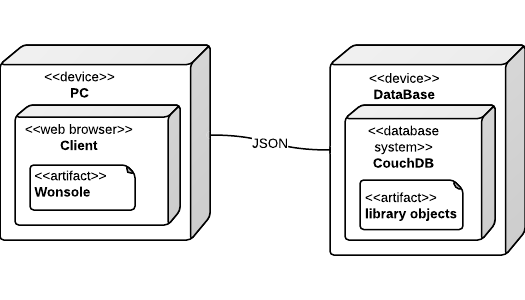
\includegraphics[width=4in]{image/architecture/s3/s3DeploymentDiagram.png}
\caption{Deployment Diagram}
\label{figure:s3DeploymentDiagram}
\end{figure}

Figure~\ref{figure:s3DeploymentDiagram} The structure of the now two different parts of the system, database can be accessed without a middleman, and the PubNub is no longer used.

\subsubsection{Development View}
Describes the system from the programmer's perspective. This will be described through how the different component parts are separated. Component and package diagrams will show this.

\begin{figure}[h]
\centering
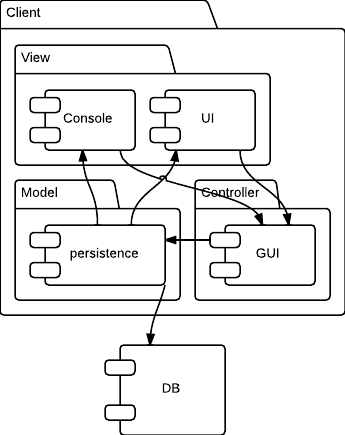
\includegraphics[width=3in]{image/architecture/s3/s3ComponentDiagram.png}
\caption{Component Diagram}
\label{figure:s3ComponentDiagram}
\end{figure}

Figure~\ref{figure:s3ComponentDiagram} These components still form a three layered structure, but the DB component is both the logical tier and the data tier. The components communicates with each other through the neighboring layer.


\section{Implementation}

\section{Testing}
\subsection{Test Results}
We performed a total of 6 test cases during this sprint; TID20-25. The results are listed in Table~\ref{table:sp3testresults}. The test cases themselves can be found in the appendix ~\ref{sec:sp3testcases}.

\begin{table}
\caption{Sprint 3 Test Results}
\centering
\begin{tabular}{ l p{13cm} }

\hline 
Item			&Description		\\
\hline \\ [-2.0ex]

\bf{TestID}		&\bf{TID20}			\\
Description	&Changing directory in the application in the console.	\\
Tester		&Øystein Heimark	\\
Date			&02/11 - 2012	\\
Result		&Success				\\
\hline \\ [-2.0ex]

\bf{TestID}		&\bf{TID21}			\\
Description	&Storing objects as local variable.  	\\
Tester		&Øystein Heimark	\\
Date			&02/11 - 2012	\\
Result		&Success			\\
\hline \\ [-2.0ex]

\bf{TestID}		&\bf{TID22}			\\
Description	&Allow for the use of functions on the objects.	\\
Tester		&Øystein Heimark	\\
Date			&02/11 - 2012	\\
Result		&Success			\\
\hline \\ [-2.0ex]

\bf{TestID}		&\bf{TID23}			\\
Description	&Allow for editing and adding of attributes.	\\
Tester		&Øystein Heimark	\\
Date			&02/11 - 2012	\\
Result		&Failure. It is not possible to add attributes from the GUI			\\
\hline \\ [-2.0ex]

\bf{TestID}		&\bf{TID24}			\\
Description	&Update GUI according to changes.	\\
Tester		&Øystein Heimark	\\
Date			&02/11 - 2012	\\
Result		&Success		'	\\
\hline \\ [-2.0ex]

\bf{TestID}		&\bf{TID25}			\\
Description	&Store changes to database.\\
Tester		&Øystein Heimark	\\
Date			&02/11 - 2012	\\
Result		&Success			\\
\hline

\end{tabular}
\label{table:sp3testresults}
\end{table}

\subsection{Test Evaluation}
We had one failed test this time, which was due to some missing functionality in the GUI. More specificly it is not possible to add new attributes to existing objects from the GUI. We decided not to correct this, as the focus of this project is the console and its functionality. We prioritized to implement more functionality to the console instead. This was a feeling shared by the customer, they wanted us to exhibit what was possible to do in the console. The functionality of the GUI was not important to them.

\section{Customer Feedback}
This sections covers the feedback we got from the customer, both before and after the sprint.
\newline
\newline
At the end of sprint 2 the customer representative informed us that he would have a meeting with others in the company, to try to identify what our product was missing, a x- factor that would appeal to the users and promote the console. At the Scrum meeting for the third sprint he announced that they had indeed found this x- factor. He wanted us to return to the roots of the project, namely adding scripting to a web- page. We should focus on adding functionality which is impossible or difficult and time consuming to do in a regular GUI.
\newline
\newline
He wanted us to add functionality that would show of the advantages of the technologies we are using, and how it would not be possible to do this with more traditional technologies. He listed some general use cases he wanted us to implement, and suggested that we looked into another solution for the backend. This was because he felt that this solution was better suited for the use cases he now presented us. He was aware of the time constraints of the project and did not expect us to manage to implement all the functionality he mentioned. But it was important that we could document that it would be possible to implement it with the technologies we are using in this project.
\newline
\newline
In the middle of the sprint we did a technology preview for the customer. The purpose of this meeting was to ensure that we were going in the right direction. We presented the user stories we had derived from the new requirements and the customer was all in all happy with these. The customer suggested that we should focus on core functionality, features that will stand out during the presentation of the project. We also presented him what we had implemented so far, including an early implementation of the CouchDB system and an early draft of the GUI. He was impressed what we had managed to implement so far, and encouraged us to keep up the good work.
\newline
\newline
At the end of the sprint we did a sprint demonstration were we presented our results to the customer. He was very happy with our progress, and didn't expect us to be able to get so far so early. For the next sprint he requested that we make a manual for how to use the system(for the users), and a deployment manual for how to set up the system on a new server(for an administrator). He also wanted us to send him a copy of our report, so he could give us some feedback on it.

\section{Evaluation}
This section contains the evaluation of the third sprint, and what we plan to improve for the fourth sprint. The evaluation was performed during an internal meeting with all group members present.

\subsection{Review}
Again we feel we were able to deliver a great product, and we were able to complete all the user stories in the sprint backlog. This sprint posed a different kind of challenge for us, as we decided to switch some of the technologies we were using and to redesign much of the system. This was obviously not according to plan, but we feel we rose to this challenge, adapted well and succeded in making the switch. We found time to research new technologies as well as incorporating these into the design of the system.
\newline
\newline
The communication with the customer was good throughout this sprint, even better than in the previous sprints. The customer was more included in the planning of this sprint, and he was more specific in what he wanted to be implemented. This helped us a lot when we were creating new user stories. This time we were also able to schedule a meeting with the customer in the middle of the sprint, to allow him a chance to provide some feedback on the prelimanary solutions we had implemented so far. We feel this great communication was reflected by the fact that the customer was very happy with the end result, which exceeded his expectations.
\newline
\newline
In previous sprints, not enough focus was put on the report and general documentation. To address this issue we decided to put two team members full time on the report for the last week of this sprint, and it resulted in more work being done with the documentation. We were able to document our work on the research and implementation effectively during the sprint, and also found time to fix some parts of the report according to feedback we recieved from the advisor. All in all we feel this was a successful move.
\newline
\newline
Despite it beeing a successful sprint in many ways, there was still some aspects of it that was not so good. In this sprint we were too dependent on one person for the implementation. We planned to assign two team members to the implementation, but one of them ended up working on the report instead. Although the person responsible for the implementation did a fantastic job, and we ended up delivering a great product, we should have done a better job in distributing the workload of the implementation. If the one assigned to the implementation somehow would be unable to work the last couple of days, we would have been in big trouble. We should have at least two team members involved in the implementation, to avoid one single point of failure.
\newline
\newline
We also fell back to our old habits with the time tracking. Our focus was disturbed by the change of direction in the project, and in the middle of it all we forgot to follow up on our routines on time tracking. We also failed to peform the test cases earlier, as we set out to do before the sprint. This may also be credited to the changes. We ended up being very pressed on time towards the end of the sprint and prioritised to complete the implementation instead.

\subsubsection{Positive}

\begin{itemize}
\item Was able to switch technologies without too many complications
\item Finished all the user stories on time
\item Great contact with the customer throughout the sprint
\item Better preparation for customer demonstration
\item Was able to create small and precise user stories, which was easier to estimate
\end{itemize}

\subsubsection{Negative}

\begin{itemize}
\item Too dependent on one person with implementation
\item Time tracking, returned to our bad habits from sprint 1
\item Failed to perform tests earlier, as we planned.
\end{itemize}

\subsection{Planned Responses}
These are the actions we have planned for the final sprint to improve our work process.

\subsubsection{Workload Distribution}
Continue the success of putting two team members full time on the report, as this turned out to be a great measure to ensure the quality of the report. Although there is not a whole lot left to do on the implementation, we should assign two people to the tasks remaining. This to avoid a potensial single point of failure.

\subsubsection{Time Tracking}
Return to our routines for time tracking, which we were able to do so well in the second sprint.


